\documentclass[]{article} 

\usepackage{tikz,pgfplots,pgfplotstable}
\usepackage{amsmath}
\usepackage{graphicx}
\usepackage{float}

\pgfplotsset{compat=newest}

\usepgfplotslibrary{statistics}
\usetikzlibrary{shapes,arrows, arrows.meta, shapes, positioning}
\usetikzlibrary{pgfplots.statistics} 

\newcommand{\findmin}[3]{
    \pgfplotstablevertcat{\datatable}{#1}
    \pgfplotstablecreatecol[
      create col/expr={%
    \pgfplotstablerow
    }]{rownumber}\datatable
    \pgfplotstablesort[sort key={#2},sort cmp={float <}]{\sorted}{\datatable}%
    \pgfplotstablegetelem{0}{rownumber}\of{\sorted}%
    \pgfmathtruncatemacro#3{\pgfplotsretval}
    \pgfplotstableclear{\datatable}
}

\pgfplotsset{
	box plot/.style={
		/pgfplots/.cd,
		black,
		only marks,
		mark=-,
		mark size=1em,
		/pgfplots/error bars/.cd,
		y dir=plus,
		y explicit,
	},
	box plot box/.style={
		/pgfplots/error bars/draw error bar/.code 2 args={%
			\draw  ##1 -- ++(1em,0pt) |- ##2 -- ++(-1em,0pt) |- ##1 -- cycle;
		},
		/pgfplots/table/.cd,
		y index=2,
		y error expr={\thisrowno{3}-\thisrowno{2}},
		/pgfplots/box plot
	},
	box plot top whisker/.style={
		/pgfplots/error bars/draw error bar/.code 2 args={%
			\pgfkeysgetvalue{/pgfplots/error bars/error mark}%
			{\pgfplotserrorbarsmark}%
			\pgfkeysgetvalue{/pgfplots/error bars/error mark options}%
			{\pgfplotserrorbarsmarkopts}%
			\path ##1 -- ##2;
		},
		/pgfplots/table/.cd,
		y index=4,
		y error expr={\thisrowno{2}-\thisrowno{4}},
		/pgfplots/box plot
	},
	box plot bottom whisker/.style={
		/pgfplots/error bars/draw error bar/.code 2 args={%
			\pgfkeysgetvalue{/pgfplots/error bars/error mark}%
			{\pgfplotserrorbarsmark}%
			\pgfkeysgetvalue{/pgfplots/error bars/error mark options}%
			{\pgfplotserrorbarsmarkopts}%
			\path ##1 -- ##2;
		},
		/pgfplots/table/.cd,
		y index=5,
		y error expr={\thisrowno{3}-\thisrowno{5}},
		/pgfplots/box plot
	},
	box plot median/.style={
		/pgfplots/box plot
	}
}

% \begin{filecontents}{testdata.dat}
% 0 1 1.2 0.4 1.5 0.2
% 1 2 2.3 1.5 2.7 1
% 2 0.7 1.4 0.5 1.9 0.1
% \end{filecontents}

% \begin{filecontents*}{scientists.csv}
% name,surname,age
% Albert,Einstein,133
% Marie,Curie,145
% Thomas,Edison,165
% \end{filecontents*}

\begin{document}

\title{Plot generation of accepted paper of \\ \emph{Modeling of Request Cloning in Cloud Server Systems using Processor Sharing}}

\maketitle

\section*{Plots with empirical data in chronological order}

\begin{figure}[H]
	\centering
	\begin{tikzpicture}[]

\begin{axis}[%
width=0.70\columnwidth,
height=0.35\columnwidth,
scale only axis,
separate axis lines,
xmin=0, xmax=8,
ymin=0, ymax=1,
xlabel = {Response time (s)},
compat = 1.4,
ylabel = {Empirical CDF},
grid style = {dashed, black!20},
grid=major,
legend columns=1,
legend style={draw, fill=white},
legend pos = south east,
ylabel near ticks,
xlabel near ticks,
legend cell align={left},
]

\addplot [color=black, thick, solid]
table [col sep=comma] {data/gg1-example-compressed/3dist-ps.csv};
\addlegendentry{Three Servers with Cloning};

\addplot [color=red, ultra thick, dashed]
table [col sep=comma] {data/gg1-example-compressed/equivalent-ps.csv};
\addlegendentry{Equivalent Single Server};

\end{axis}
\end{tikzpicture}
	\caption{Empirical response time CDFs for the Example with Heterogeneous Servers. Data retrieved through 20 repeated simulations of $10^6$ requests each. The 95\% confidence intervals lie within the lines.}
	\label{fig:gg1-results-ps}
\end{figure}


\begin{figure}[H]
	\centering
	\begin{tikzpicture}[]
\pgfplotsset{set layers}

\begin{axis}[%
width=0.75\columnwidth,
height=0.40\columnwidth,
scale only axis,
separate axis lines,
xmin=0,
xmax=0.7,
ymin=0,
ymax=10,
axis y line*=right,
axis x line=none,
ytick={2, 4, 6, 8, 10},
compat=1.4,
ylabel={$\mathbf{E}[T]$ (s)},
grid style={dashed,black!20},
grid=major,
legend columns=1,
legend style={draw, fill=white, at={(0.98, 0.98)}, anchor=north east},
ylabel near ticks,
xlabel near ticks,
legend cell align={left},
]

\addplot [color=black, thick, solid]
table [col sep=comma] {data/clone-to-all-compressed/meanRTs-ps.csv};
\addlegendentry{$\mathbf{E}[T]^{\text{opt}}$ (theory)}

%\addplot [color=green, thick, dashed]
%table [col sep=comma] {data/clone-to-all/minAvgRTVal-mean-ps.csv};
%\addlegendentry{$\mathbf{E}[T]^{\text{opt}}$ (sim)}

\addplot[area legend,dashed,fill=green,draw=green,opacity=5e-01]
table [col sep=comma]
{data/clone-to-all/optmean-confint.csv};
\addlegendentry{$\mathbf{E}[T]^{\text{opt}}$ (sim)}

\draw[->, >=latex, thick] (axis cs:0.52, 5.75) -- (axis cs:0.57, 5.75);

\end{axis}

\begin{axis}[%
width=0.75\columnwidth,
height=0.40\columnwidth,
scale only axis,
separate axis lines,
axis y line*=left,
xmin=0,
xmax=0.7,
ymin=0,
ymax=10,
xlabel={Arrival rate / server (1/s)},
compat=1.4,
ylabel={Cloning factor $c_f$},
grid style={dashed,black!20},
grid=major,
legend columns=1,
legend style={draw, fill=white, at={(0.02, 0.15)}, anchor=south west},
ylabel near ticks,
xlabel near ticks,
legend cell align={left},
]

%\addplot[area legend,solid,fill=black,opacity=2.5e-01,draw=none]
%table [col sep=comma] {data/clone-to-all/minAvgRTSer_minmax.csv};
%\addlegendentry{minmax};

\addplot [color=red, thick, solid]
table [col sep=comma] {data/clone-to-all-compressed/optclones-ps.csv};
\addlegendentry{$c_f^{\text{opt}}$ (theory)};

%\addplot [color=blue, thick, dashed]
%table [col sep=comma] {data/clone-to-all/minAvgRTSer-mean-ps.csv};
%\addlegendentry{$c_f^{\text{opt}}$ (sim)};

\addplot[area legend,dashed,fill=blue,draw=blue,opacity=5e-01]
table [col sep=comma] {data/clone-to-all/optclone-confint.csv};
\addlegendentry{$c_f^{\text{opt}}$ (sim)};

%\addplot [color=black, thick, dashed]
%table [col sep=comma] {data/clone-to-all/minAvgRTSer_min.csv};

%\addplot [color=black, thick, dashed]
%table [col sep=comma] {data/clone-to-all/minAvgRTSer_max.csv};

\draw[->, >=latex, thick] (axis cs:0.1, 5.75) -- (axis cs:0.05, 5.75);

\end{axis}

\end{tikzpicture}%
	\caption{Clone-to-All: Comparison of theoretical values with 95\% confidence intervals for the simulation results.}
	\label{fig:clone-to-all-evaluation}
\end{figure}

  \begin{figure}[H]
	\centering
	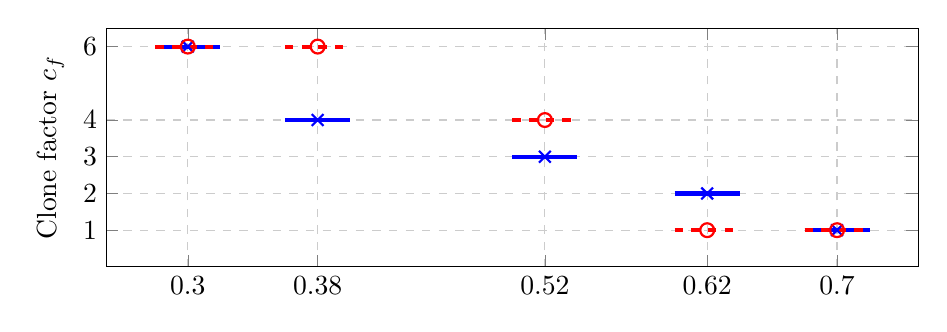
\begin{tikzpicture}

\begin{axis}[%
width=0.85\columnwidth,
height=0.25\columnwidth,
scale only axis,
xmin=0.25,
xmax=0.75,
xtick={0.3, 0.38, 0.52, 0.62, 0.70},
ymin=0,
ymax=6.5,
ytick={1, 2, 3, 4, 6},
ylabel={Clone factor $c_f$},
grid style={dashed,black!20},
grid=major,
legend columns=2,
legend style={draw, fill=white, at={(0.01, 0.05)}, anchor=south west},
ylabel near ticks,
xlabel near ticks,
legend cell align={left},
]

\addplot[solid, blue, line width=1.5pt]
  table[row sep=crcr]{%
x y\\
0.28 6\\
0.32 6\\
};
%\addlegendentry{c-JSQ-d}

\addplot[blue,mark=x,mark options=solid, only marks,mark size=3pt, thick]
  table[row sep=crcr]{%
x y\\
0.30 6\\
0.38 4\\
0.52 3\\
0.62 2\\
0.70 1\\
};
%\addlegendentry{theory}

\addplot[solid, blue, line width=1.5pt, forget plot]
  table[row sep=crcr]{%
x y\\
0.36 4\\
0.40 4\\
};

\addplot[solid, blue, line width=1.5pt, forget plot]
  table[row sep=crcr]{%
x y\\
0.50 3\\
0.54 3\\
};

\addplot[solid, blue, line width=1.5pt, forget plot]
  table[row sep=crcr]{%
x y\\
0.60 2\\
0.64 2\\
};

\addplot[solid, blue, line width=1.5pt, forget plot]
  table[row sep=crcr]{%
x y\\
0.68 1\\
0.72 1\\
};

\addplot[dashed, red, line width=1.5pt]
  table[row sep=crcr]{%
x y\\
0.28 6\\
0.32 6\\
};
%\addlegendentry{c-R-d}

\addplot[red,mark=o, only marks,mark size=2.5pt, thick]
  table[row sep=crcr]{%
x y\\
0.30 6\\
0.38 6\\
0.52 4\\
0.62 1\\
0.70 1\\
};
%\addlegendentry{theory}

\addplot[dashed, red, line width=1.5pt, forget plot]
  table[row sep=crcr]{%
x y\\
0.36 6\\
0.40 6\\
};

\addplot[dashed, red, line width=1.5pt, forget plot]
  table[row sep=crcr]{%
x y\\
0.50 4\\
0.54 4\\
};

\addplot[dashed, red, line width=1.5pt, forget plot]
  table[row sep=crcr]{%
x y\\
0.60 1\\
0.64 1\\
};

\addplot[dashed, red, line width=1.5pt, forget plot]
  table[row sep=crcr]{%
x y\\
0.68 1\\
0.72 1\\
};

\end{axis}
\end{tikzpicture}
	
	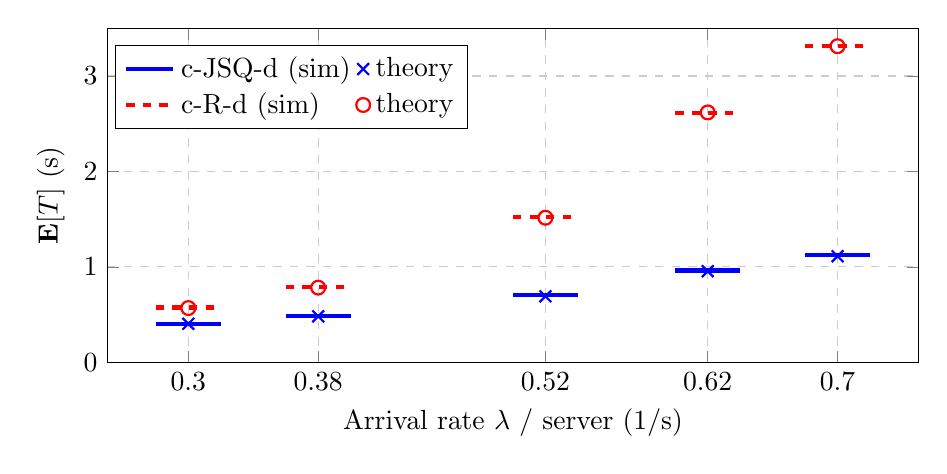
\begin{tikzpicture}


\begin{axis}[%
width=0.85\columnwidth,
height=0.35\columnwidth,
scale only axis,
separate axis lines,
xmin=0.25,
xmax=0.75,
xlabel={Arrival rate $\lambda$ / server (1/s)},
xtick={0.3, 0.38, 0.52, 0.62, 0.70},
ymin=0,
ymax=3.5,
ytick={0,1,2,3},
ylabel={$\mathbf{E}[T]$ (s)},
grid style={dashed,black!20},
grid=major,
legend columns=2,
legend style={draw, fill=white, at={(0.01, 0.95)}, anchor=north west},
ylabel near ticks,
xlabel near ticks,
legend cell align={left},
]

\addplot[solid, blue, line width=1.5pt]
  table[row sep=crcr]{%
x y\\
0.28 0.4053\\
0.32 0.4053\\
};
\addlegendentry{c-JSQ-d (sim)}

\addplot[blue,mark=x,mark options=solid, only marks,mark size=3pt, thick]
  table[row sep=crcr]{%
x y\\
0.30 0.404\\
0.38 0.482\\
0.52 0.692\\
0.62 0.955\\
0.70 1.112\\
};
\addlegendentry{theory}

\addplot[solid, blue, line width=1.5pt, forget plot]
  table[row sep=crcr]{%
x y\\
0.36 0.4868\\
0.40 0.4868\\
};

\addplot[solid, blue, line width=1.5pt, forget plot]
  table[row sep=crcr]{%
x y\\
0.50 0.7067\\
0.54 0.7067\\
};

\addplot[solid, blue, line width=1.5pt, forget plot]
  table[row sep=crcr]{%
x y\\
0.60 0.9631\\
0.64 0.9631\\
};

\addplot[solid, blue, line width=1.5pt, forget plot]
  table[row sep=crcr]{%
x y\\
0.68 1.1223\\
0.72 1.1223\\
};

\addplot[dashed, red, line width=1.5pt]
  table[row sep=crcr]{%
x y\\
0.28 0.5743\\
0.32 0.5743\\
};
\addlegendentry{c-R-d (sim)}

\addplot[red,mark=o, only marks,mark size=2.5pt, thick]
  table[row sep=crcr]{%
x y\\
0.30 0.569\\
0.38 0.783\\
0.52 1.515\\
0.62 2.618\\
0.70 3.312\\
};
\addlegendentry{theory}

\addplot[dashed, red, line width=1.5pt, forget plot]
  table[row sep=crcr]{%
x y\\
0.36 0.7879\\
0.40 0.7879\\
};

\addplot[dashed, red, line width=1.5pt, forget plot]
  table[row sep=crcr]{%
x y\\
0.50 1.5185\\
0.54 1.5185\\
};

\addplot[dashed, red, line width=1.5pt, forget plot]
  table[row sep=crcr]{%
x y\\
0.60 2.6154\\
0.64 2.6154\\
};

\addplot[dashed, red, line width=1.5pt, forget plot]
  table[row sep=crcr]{%
x y\\
0.68 3.3176\\
0.72 3.3176\\
};
\end{axis}
\end{tikzpicture}
	\caption{Co-designs: Comparison of theoretical values with 95\% confidence intervals for the simulation results. The legend applies to both figures.}
	\label{fig:co-design}
\end{figure}

\begin{figure}[H] 
	\centering
	\begin{tikzpicture}


\begin{axis}[%
width=0.82\columnwidth,
height=3.0cm,
scale only axis,
separate axis lines,
%no markers,
xmin=0.006,
xmax=0.8,
xlabel={$\frac{\mathbf{E}[a]}{\mathbf{E}[X]}$},
ylabel={Normalized $\mathbf{E}[T]$},
xmode=log,
xtick = data,
log ticks with fixed point,
%symbolic x coords={0.05, 0.10, 0.20, 0.50},
%xticklabels = {0.05, 0.10, 0.20, 0.50},
%xtick={0.1, 0.2, 0.3, 0.4, 0.5, 0.6, 0.7, 0.8, 0.9},
ymin=0.99,
%xlabel={Utilization $\rho$},
ymax=1.3,
ytick={1, 1.05, 1.1, 1.15, 1.20, 1.25, 1.3},
yticklabels = {1,, 1.1,, 1.2,, 1.3},
compat=1.5.1,
%ylabel={ $\mathbf{E}[T^{ns}]/\mathbf{E}[T^{s}]$},
grid style={dashed,black!20},
grid=major,
legend columns=1,
legend style={draw, fill=white, at={(0.02, 0.95)}, anchor=north west},
ylabel near ticks,
xlabel near ticks,
legend cell align={left},
]

\addplot+[red, only marks, mark options={red}, mark size=1.5pt,
  error bars/.cd,
    y dir=both,
    y explicit,
    error bar style={line width=1pt},
    error mark options={
      rotate=90,
      mark size=6pt,
      line width=1pt
    }
]
table [x index=0, y index=2, x error index=1, y error index=3] {data/randomized-delays/randomized_arrival_delays_confint_bound.txt};
\addlegendentry{Upper bound}

\addplot+[blue, only marks, mark options={blue}, mark size=1.5pt,
  error bars/.cd,
    y dir=both,
    y explicit,
    error bar style={line width=1pt},
    error mark options={
      rotate=90,
      mark size=6pt,
      line width=1pt
    }
]
table [x index=0, y index=2, x error index=1, y error index=3] {data/randomized-delays/randomized_arrival_delays_confint_resp.txt};
\addlegendentry{Delays}

\addplot[dashed, black, line width=1.0pt]
  table[row sep=crcr]{%
x y\\
0.005 1\\
0.8 1\\
};
\addlegendentry{No delays}

\end{axis}
\end{tikzpicture}
	\caption{Arrival delays only.}
\end{figure}

\begin{figure}[H]
	\centering
	\begin{tikzpicture}


\begin{axis}[%
width=0.82\columnwidth,
height=3.0cm,
scale only axis,
separate axis lines,
%no markers,
xmin=0.006,
xmax=0.8,
xlabel={$\frac{\mathbf{E}[c]}{\mathbf{E}[X]}$},
ylabel={Normalized $\mathbf{E}[T]$},
xmode=log,
xtick = data,
log ticks with fixed point,
%symbolic x coords={0.05, 0.10, 0.20, 0.50},
%xticklabels = {0.05, 0.10, 0.20, 0.50},
%xtick={0.1, 0.2, 0.3, 0.4, 0.5, 0.6, 0.7, 0.8, 0.9},
ymin=0.95,
%xlabel={Utilization $\rho$},
ymax=2.90,
%ytick={0, 0.2, 0.4, 0.6, 0.8, 1.0},
compat=1.5.1,
%ylabel={ $\mathbf{E}[T^{ns}]/\mathbf{E}[T^{s}]$},
grid style={dashed,black!20},
grid=major,
legend columns=1,
legend style={draw, fill=white, at={(0.02, 0.95)}, anchor=north west},
ylabel near ticks,
xlabel near ticks,
legend cell align={left},
]

\addplot+[red, only marks, mark options={red}, mark size=1.5pt,
  error bars/.cd,
    y dir=both,
    y explicit,
    error bar style={line width=1pt},
    error mark options={
      rotate=90,
      mark size=6pt,
      line width=1pt
    }
]
table [x index=0, y index=2, x error index=1, y error index=3] {data/randomized-delays/randomized_cancellation_delays_confint_bound.txt};
%\addlegendentry{Upper bound}

\addplot+[blue, only marks, mark options={blue}, mark size=1.5pt,
  error bars/.cd,
    y dir=both,
    y explicit,
    error bar style={line width=1pt},
    error mark options={
      rotate=90,
      mark size=6pt,
      line width=1pt
    }
]
table [x index=0, y index=2, x error index=1, y error index=3] {data/randomized-delays/randomized_cancellation_delays_confint_resp.txt};
%\addlegendentry{Delays}

\addplot[dashed, black, line width=1.0pt]
  table[row sep=crcr]{%
x y\\
0.005 1\\
0.8 1\\
};
%\addlegendentry{No delays}

\end{axis}
\end{tikzpicture}
	\caption{Cancellation delays only.}
\end{figure}

\begin{figure}[H]
	\centering
	\begin{tikzpicture}


\begin{axis}[%
width=0.82\columnwidth,
height=3.0cm,
scale only axis,
separate axis lines,
%no markers,
xmin=0.006,
xmax=0.8,
xlabel={$\frac{\mathbf{E}[a+c]}{\mathbf{E}[X]}$},
ylabel={Normalized $\mathbf{E}[T]$},
xmode=log,
xtick = data,
log ticks with fixed point,
%symbolic x coords={0.05, 0.10, 0.20, 0.50},
%xticklabels = {0.05, 0.10, 0.20, 0.50},
%xtick={0.1, 0.2, 0.3, 0.4, 0.5, 0.6, 0.7, 0.8, 0.9},
ymin=0.95,
%xlabel={Utilization $\rho$},
ymax=2.90,
%ytick={0, 0.2, 0.4, 0.6, 0.8, 1.0},
compat=1.5.1,
%ylabel={ $\mathbf{E}[T^{ns}]/\mathbf{E}[T^{s}]$},
grid style={dashed,black!20},
grid=major,
legend columns=1,
legend style={draw, fill=white, at={(0.02, 0.95)}, anchor=north west},
ylabel near ticks,
xlabel near ticks,
legend cell align={left},
]

\addplot+[red, only marks, mark options={red}, mark size=1.5pt,
  error bars/.cd,
    y dir=both,
    y explicit,
    error bar style={line width=1pt},
    error mark options={
      rotate=90,
      mark size=6pt,
      line width=1pt
    }
]
table [x index=0, y index=2, x error index=1, y error index=3] {data/randomized-delays/randomized_combined_delays_confint_bound_v2.txt};
%\addlegendentry{Upper bound}

\addplot+[blue, only marks, mark options={blue}, mark size=1.5pt,
  error bars/.cd,
    y dir=both,
    y explicit,
    error bar style={line width=1pt},
    error mark options={
      rotate=90,
      mark size=6pt,
      line width=1pt
    }
]
table [x index=0, y index=2, x error index=1, y error index=3] {data/randomized-delays/randomized_combined_delays_confint_resp_v2.txt};
%\addlegendentry{Delays}

\addplot[dashed, black, line width=1.0pt]
  table[row sep=crcr]{%
x y\\
0.005 1\\
0.8 1\\
};
%\addlegendentry{No delays}

\end{axis}
\end{tikzpicture}
	\caption{Both delays present.}
\end{figure}

\begin{figure}[H]
	\centering
	\begin{tikzpicture}


\begin{axis}[%
width=0.85\columnwidth,
height=0.30\columnwidth,
scale only axis,
separate axis lines,
%no markers,
xmin=0.05,
xmax=0.95,
xtick={0.1, 0.2, 0.3, 0.4, 0.5, 0.6, 0.7, 0.8, 0.9},
ymin=0.0,
ymax=0.33,
%ytick={0, -0.1,-0.2, -0.3, -0.4, -0.5, -0.6},
compat=1.5.1,
ylabel={$\mathbf{E}[\epsilon]$},
grid style={dashed,black!20},
grid=major,
legend columns=1,
legend style={draw, fill=white, at={(0.05, 0.95)}, anchor=north west},
ylabel near ticks,
xlabel near ticks,
legend cell align={left},
]

\addplot+[color=blue, only marks, mark=*, mark size=1.5pt,
  error bars/.cd,
    y dir=both,
    y explicit,
    error bar style={line width=1pt},
    error mark options={
      rotate=90,
      mark size=6pt,
      line width=1pt
    }
]
table [x index=0, y index=2, x error index=1, y error index=3] {data/randomized-sync-vs-nonsync/randomized_sqf_clone_confint.txt};
\addlegendentry{a-JSQ-d}

\addplot+[color=red, only marks, mark=square*, mark size=1.5pt,
  error bars/.cd,
    y dir=both,
    y explicit,
    error bar style={line width=1pt},
    error mark options={
      rotate=90,
      mark size=6pt,
      line width=1pt
    }
]
table [x index=0, y index=2, x error index=1, y error index=3] {data/randomized-sync-vs-nonsync/randomized_random_clone_confint.txt};
\addlegendentry{a-R-d}


\end{axis}
\end{tikzpicture}
	
	\begin{tikzpicture}


\begin{axis}[%
width=0.85\columnwidth,
height=0.47\columnwidth,
scale only axis,
separate axis lines,
%no markers,
xmin=0.05,
xmax=0.95,
xtick={0.1, 0.2, 0.3, 0.4, 0.5, 0.6, 0.7, 0.8, 0.9},
ymin=0.38,
xlabel={Utilization $\rho$},
ymax=1.02,
ytick={0.4, 0.5, 0.6, 0.7, 0.8, 0.9, 1},
compat=1.5.1,
ylabel={Normalized $\mathbf{E}[T]$},
grid style={dashed,black!20},
grid=major,
legend columns=1,
legend style={draw, fill=white, at={(0.05, 0.05)}, anchor=south west},
ylabel near ticks,
reverse legend,
xlabel near ticks,
legend cell align={left},
]

\addplot[dashed, black, line width=1.0pt]
  table[row sep=crcr]{%
x y\\
0.0 1\\
1.0 1\\
};
\addlegendentry{c-$\ell$-d}

\addplot+[red, only marks, mark options={red}, mark size=1.5pt,
  error bars/.cd,
    y dir=both,
    y explicit,
    error bar style={line width=1pt},
    error mark options={
      rotate=90,
      mark size=6pt,
      line width=1pt
    }
]
table [x index=0, y index=2, x error index=1, y error index=3] {data/randomized-sync-vs-nonsync/randomized_random_mean_confint.txt};
\addlegendentry{a-R-d}

\addplot+[blue, only marks, mark options={blue}, mark size=1.5pt,
  error bars/.cd,
    y dir=both,
    y explicit,
    error bar style={line width=1pt},
    error mark options={
      rotate=90,
      mark size=6pt,
      line width=1pt
    }
]
table [x index=0, y index=2, x error index=1, y error index=3] {data/randomized-sync-vs-nonsync/randomized_sqf_mean_confint.txt};
\addlegendentry{a-JSQ-d}


\end{axis}
\end{tikzpicture}
	\caption{Simulations comparing a-$\ell$-d to c-$\ell$-d for random and JSQ. The normalization of $\mathbf{E}[T]$ is performed such that each value is divided by the value for the c-$\ell$-d counterpart. The intervals represent 95\% confidence intervals.}
	\label{fig:nonsync-vs-sync}
\end{figure}

\end{document}
